\chapter{Math Operators and Libraries}\label{CHAP_MathOperators}

\section{Difficulty: EASY}

\subsubsection*{Exercise 4.E01}
Determine the result of:
\begin{enumerate}[label=(\alph*)]
	\item $15 + 35.6 + 20.78 - 0.01$
	\item $0.5 + (0.8 \cdot 0.5) - 0.333$
	\item $(0.5 + 0.8) \cdot (0.5 - 0.333)$
	\item $100 / (400 \cdot 4)$
	\item $100/ 400 \cdot 4$
	\item $2.0^5 + 100$
	\item $2.0^{(5 + 100)}$
\end{enumerate}

\textit{Hints:
Use the addition $+$, subtraction $-$, multiplication *, division $/$ and exponent ** operators. Remember that brackets can change the order in which mathematical expressions are evaluated.}\\[1cm]


% ------------------------------------------------------------------------------

\newpage
\subsubsection*{Exercise 4.E02}
Copy the following definitions into Jupyter Notebook:
\begin{figure}[H]
		\centering
		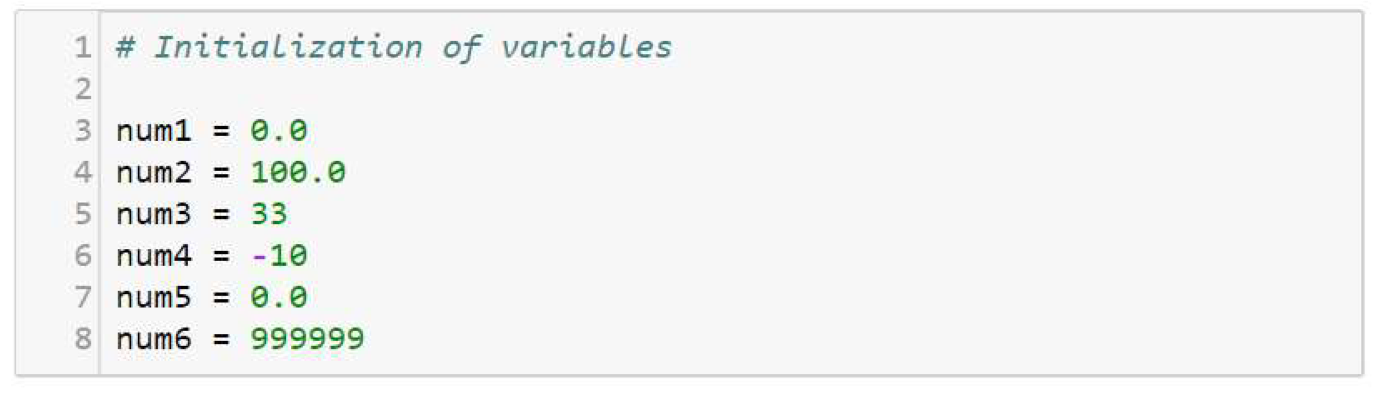
\includegraphics[width=\textwidth]{../IMG/4E02.png} 
\end{figure}


Using comparison operators, determine whether:
\begin{enumerate}[label=(\alph*)]
	\item {\code{num1}} is smaller than {\code{num3}}
	\item {\code{num2}} is smaller than or equal to {\code{num6}}
	\item {\code{num3}} is larger than {\code{num4}}
	\item {\code{num5}} is larger than or equal to {\code{num6}}
	\item {\code{num5}} and {\code{num1}} are the same
	\item {\code{num2}} and {\code{num4}} are not the same
\end{enumerate}

\textit{Hints:
Use the comparison operators $<$, $<=$, $>$, $>=$, $==$, and $!=$. Remember that $=$ is a declaration and $==$ a comparison!}\\[1cm]


% ------------------------------------------------------------------------------

\subsubsection*{Exercise 4.E03}
In this exercise you will be using functions defined in the math library. To use them in your
own code, you will first need to import the library with the following syntax:
\begin{center}
	{\code{import math}}
\end{center}
Copy the following variable declarations into a Jupyter Notebook
\begin{figure}[H]
		\centering
		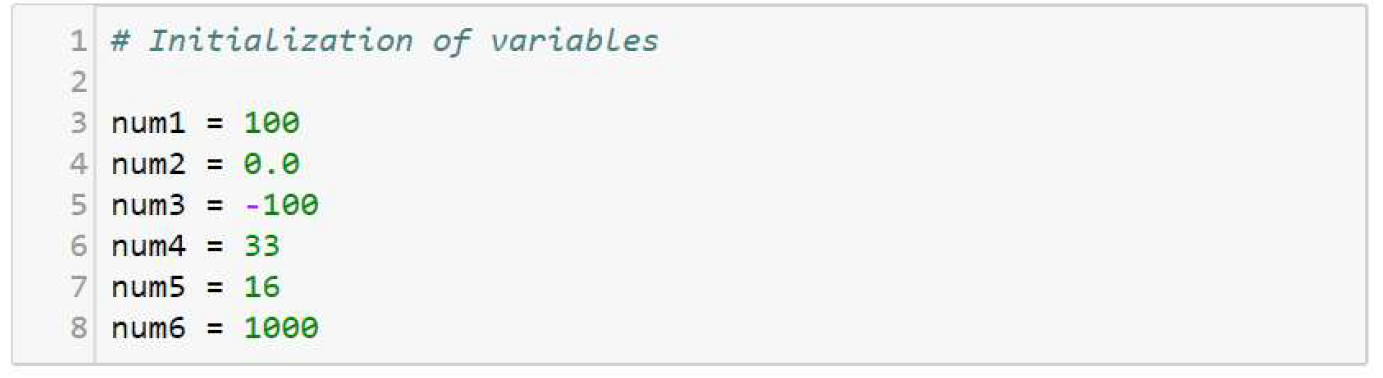
\includegraphics[width=\textwidth]{../IMG/4E03.png} 
\end{figure}

then
\begin{enumerate}[label=(\alph*)]
	\item Calculate the square root of {\code{num1}}
	\item Calculate the square root of {\code{num4}}
	\item Calculate the absolute value of {\code{num5}}
	\item Calculate the absolute value of {\code{num3}}
	\item Determine whether the absolute values of {\code{num1}} and {\code{num3}} are the same
	\item Determine whether the square root of {\code{num6}} is larger than {\code{num1}}
	\item Determine whether the absolute value of {\code{num5}} is smaller than {\code{num2}}
	\item Determine whether the square root of the sum of {\code{num1}} and {\code{num2}} is larger than 200
	\item Determine the multiplication product of the square root of {\code{num5}} and the absolutevalue of {\code{num3}}
	\item Determine the square root of the square root of {\code{num5}}
\end{enumerate}


\textit{Hints:
To use a function from a library you follow the syntax\\
\begin{center}
	{\code{libraryName.functionName(arguments)}}.
\end{center}
In this exercise you will need the math.sqrt(x) function to calculate the square root of {\code{x}} and the {\code{math.fabs(x)}} function to calculate the absolute value of {\code{x}}.
Remember: You can compare numbers using the comparison operators which will return a Boolean to you. You can also carry out operation in between the brackets of a function.}\\[1cm]


% ------------------------------------------------------------------------------

\subsubsection*{Exercise 4.E04 \red{[M]}}
Translate the mathematical notations used below into familiar Python command structures
and solve the equations
\begin{enumerate}[label=(\alph*)]
	\item For $x = 5$ determine the result of $y = 6x^2+3x+2$
	\item For $x = 0.5$ determine the result of $y = \sqrt{\sqrt{\sqrt{x/3.6}}}$
	\item For $a = 3$, $b = 10$, and $c = -2$ determine the two possible results of $y_{1/2} = \frac{-b \pm \sqrt{b^2-4ac}}{2a}$
\end{enumerate}

\textit{Hints:
In this exercise you will need additions $+$, subtractions $-$, multiplications *, exponents **, square roots {\code{sqrt()}} (from the math library) and divisions $/$.}


% ------------------------------------------------------------------------------


\section{Difficulty: MEDIUM}

\subsubsection*{Exercise 4.M01}
Write a code that accepts a distance and converts it from:
\begin{enumerate}[label=(\alph*)]
	\item Kilometres to miles
	\item Miles to Kilometres.
\end{enumerate}
The conversion rules are given by the following equations:\\
Conversion km to miles:
\begin{center}
	$x_{\textrm{miles}} = 0.621371 \cdot x_{\textrm{km}}$
\end{center}
Conversion miles to km:
\begin{center}
	$x_{\textrm{km}} = 1.60934 \cdot x_{\textrm{miles}}$.
\end{center}


\textit{Hints:
You will need the multiplication * operator. To check whether your code is working, you can
test it using the following website: \url{https://www.rapidtables.com/convert/length/km-tomile.
html}}\\[1cm]


% ------------------------------------------------------------------------------

\subsubsection*{Exercise 4.M02}
Write a code that accepts a temperature and converts it from:
\begin{enumerate}[label=(\alph*)]
	\item Fahrenheit to Celsius
	\item Celsius to Fahrenheit.
\end{enumerate}
The conversion rules are given by the following equations:\\
Conversion Fahrenheit to Celsius::
\begin{center}
	$T_{\textrm{Celsius}} = (T_{\textrm{Fahrenheit}}-32)\cdot 5/9$
\end{center}
Conversion Celsius to Fahrenheit::
\begin{center}
	$T_{\textrm{Fahrenheit}} = T_{\textrm{Celsius}} \cdot 9/5 + 32$.
\end{center}


\textit{Hints:
You will need the addition $+$, subtraction $-$, multiplication * and division $/$ operators. To
check whether your code is working, visit the following website:
\url{https://www.rapidtables.com/convert/temperature/celsius-to-fahrenheit.html}}\\[1cm]


% ------------------------------------------------------------------------------

\subsubsection*{Exercise 4.M03 \red{[M]}}
Using the {\code{math.pi}} constant from the {\code{math}} library, write a code that calculates
\begin{enumerate}[label=(\alph*)]
	\item The area of a circle given a radius $r$
	\item The volume of a sphere given a radius $r$.
\end{enumerate}

\begin{figure}[H]
		\centering
		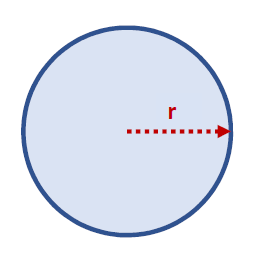
\includegraphics[width=0.3\textwidth]{../IMG/4M03_1.png} 
\end{figure}

The area $A$ of a circle is calculated via $A = \pi \cdot r^2$.


\begin{figure}[H]
		\centering
		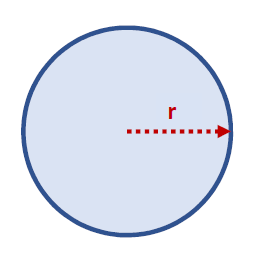
\includegraphics[width=0.3\textwidth]{../IMG/4M03_1.png} 
\end{figure}

The volume $V$ of a sphere is calculated via $V = \frac{4}{3} \cdot \pi \cdot r^3$.\\

\textit{Hints:
In addition to the {\code{math.pi}} constant, you will need the division operator $/$, the multiplication operator * and the exponent operator **. You can check your code with the following links:\\
\url{https://www.calculateme.com/cArea/AreaOfCircle.htm} (area of a circle) and
\url{https://www.calculateme.com/cVolume/VolumeOfSphere.htm} (volume of a sphere)}\\[1cm]


% ------------------------------------------------------------------------------

\subsubsection*{Exercise 4.M04}
Using compound operators, determine the results of
\begin{enumerate}[label=(\alph*)]
	\item {\code{num1 = num1 + 50}}
	\item {\code{num2 = num2 - 100}}
	\item {\code{num3 = num3 * 1000}}
	\item {\code{num4 = num4 / 10}}
	\item {\code{num4 = num4 + num1}}
\end{enumerate}	
	
\textit{Hints:
Before copying anything into your Jupyter Notebook, try rewriting the commands given in (a)
to (e) using the compound operators. Then make sure the results check out.}\\[1cm]


% ------------------------------------------------------------------------------

\subsubsection*{Exercise 4.M05 \red{[M]}}
Write a code that asks the user to provide a time duration in seconds. Convert the time into
the following format: w days, x hours, y minutes and z seconds and display the result.\\

\textit{Hints:
There are multiple ways of solving this exercise. The easiest way is via the modulus and floor
division operators from the standard Python library.\\
Using // and \% you can now approach the exercises like this:
Say T is the time in seconds given by the user.\\
\begin{enumerate}
	\item The first thing you want to do is figure our how many days are in T seconds. To do that
calculate:
\begin{center}
	{\code{days = T // (24 * 60 * 60 )}}
\end{center}
{\code{24 * 60 * 60}} are the number of seconds in one day. By calculating the floor division {\code{T // (24 * 60 * 60)}} you can determine how many full days fit into T.
Then you will need to figure out how many seconds are now left once you have removed the
seconds that correspond to full days. To do that calculate
{\code{T = T \% (24 * 60 * 60)}}
The modulus will automatically give you the remainder of the {\code{T // (24 * 60 * 60)}}
division which corresponds to the leftover seconds.
	\item The next step will determine how many hours are in the remaining T seconds. To do that
calculate:
\begin{center}
	{\code{hours = T // (60 * 60)}}
\end{center}
{\code{60 * 60}} are the number of seconds in one hour. By calculating the floor division\\
{\code{T // (60 * 60)}} you can determine how many full hours fit into T.
Then you will need to figure out how many seconds are now left once you have removed the
seconds that correspond to full hours. To do that calculate
\begin{center}
	{\code{T = T \% (60 * 60)}}
\end{center}
The modulus will automatically give you the remainder of the 
{\code{T // (60 * 60)}} division
which corresponds to the leftover seconds.
	\item Now determine the number of full minutes in the remaining seconds following the example
above. One minute contains 60 seconds.
	\item Finally, the leftover number are the remaining seconds.
\end{enumerate}
Visit: \url{https://www.tools4noobs.com/online_tools/seconds_to_hh_mm_ss/} to check whether
your code is returning the right results. }\\[1cm]


% ------------------------------------------------------------------------------

\subsubsection*{Exercise 4.S01}
Import the math library and calculate:
\begin{enumerate}[label=(\alph*)]
	\item $\sin{x}$ for $x = 0$
	\item $\sin{x}$ for $x = \frac{1}{2}\pi$
	\item $\cos{x}$ for $x = 0$
	\item $\cos{x}$ for $x = \frac{1}{2}\pi$
\end{enumerate}

\textit{Hints:
You can calculate them in Python using the {\code{math.sin()}} and {\code{math.cos()}} functions from the {\code{math}} library. The mathematical constant $\pi$ is stored in the variable math.pi from the {\code{math}} library.\\
Have a look at the documentation for the math library here:
\url{https://docs.python.org/2/library/math.html} for descriptions of the {\code{sin()}} and {\code{cos()}} functions and how to use them.}\\[1cm]


% ------------------------------------------------------------------------------

\subsubsection*{Exercise 4.S02}
Write a code that converts an angle from
\begin{enumerate}[label=(\alph*)]
	\item radians to degrees
	\item degrees to radians
\end{enumerate}
The conversion rules are as follows:\\
Conversion Radians to Degrees:
\begin{center}
	$x_{\textrm{degrees}} = \frac{360}{2\pi} \cdot x_{\textrm{radians}}$
\end{center}
Conversion Degrees to Radians:
\begin{center}
	$x_{\textrm{radians}} = \frac{2\pi}{360} \cdot x_{\textrm{degrees}}$
\end{center}

\textit{Hints:
You can look up the value of $\pi$ and declare it as a variable in your code or import it from the {\code{math}} library using {\code{math.pi}}. Have a look at the documentation for the {\code{math}} library here: \url{https://docs.python.org/2/library/math.html} for more information on the {\code{math.pi}} constant and other function included in the {\code{math}} library. To check the results, visit:\\
\url{https://www.rapidtables.com/convert/number/radians-to-degrees.html} (Radians to degrees), 
\url{https://www.rapidtables.com/convert/number/degrees-to-radians.html} (Degrees to radians).}\\[1cm]


% ------------------------------------------------------------------------------



\section{Difficulty: HARD}

\subsubsection*{Exercise 4.H01}
Look at the following code block:
\begin{figure}[H]
		\centering
		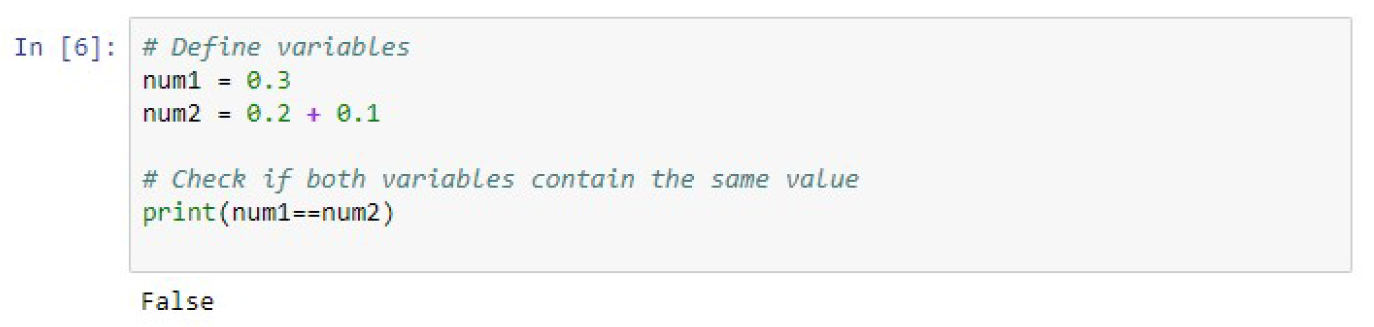
\includegraphics[width=\textwidth]{../IMG/4H01.png} 
\end{figure}
Why is the result {\code{FALSE}}? Where is the mistake coming from? How could you compare
numbers without encountering this problem?\\

\textit{Hints:
Display num1 and num2 to your screen and compare the output.}\\[1cm]


% ------------------------------------------------------------------------------

\subsubsection*{Exercise 4.H02 \red{[M]}}
Write a code that measures the distance between two points in two-dimensional space. The
coordinates of the first point are {\code{x1}} and {\code{y1}}, the coordinates of the second point are {\code{x2}} and {\code{y2}}.\\
To calculate the distance d use the following equation:

\begin{center}
$d^2 = |x1 -x2|^2 + |y1-y2|^2$
\end{center}

\begin{figure}[H]
		\centering
		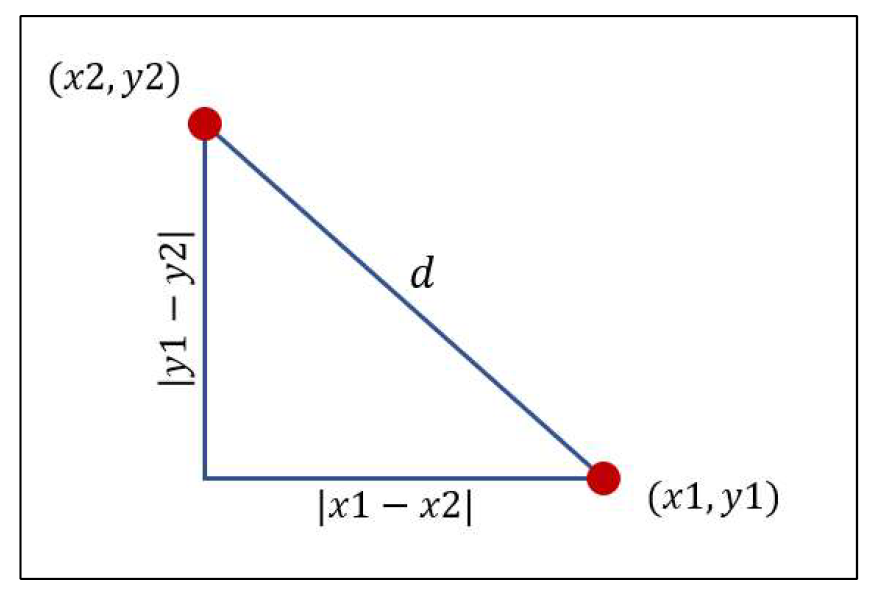
\includegraphics[width=0.5\textwidth]{../IMG/4H02.png} 
\end{figure}

Bonus:\\
Instead of hard coding the coordinates into your code ask the user to provide them in the
following format: {\code{(x, y)}}. Extract the coordinate information from the user input using
string operators and calculate the distance.\\


\textit{Hints:
You will need the {\code{math.fabs()}} and the {\code{math.sqrt()}} functions from the {\code{math library}}.\\
For the bonus exercise:\\
Try and identify a pattern in the input format and then find a way to extract information
from the string. Remember you can use the find() function to search for characters in a
string. {\code{str[i:j]}} will generate a substring from string str ranging from index {\code{i}} up to but excluding index {\code{j}}. To convert a string into a number use the {\code{str()}} function.}\\[1cm]


% ------------------------------------------------------------------------------

\subsubsection*{Exercise 4.H03 \red{[M]}}
Have a look at the figure below
A swimmer at position $A$ wants to cross the river of width $w$. The swimmer can swim with a
constant velocity $v_{\textrm{Swimmer}}$ but only along the $x$-axis. The water itself flows with velocity $v_{\textrm{Water}}$ along the $y$-axis. Once the swimmer enters the water at position $A (0,5)$ and starts to cross the river, the water will carry them downstream with respect to $A$. Write a code that calculates the position $B$ at which the swimmer reaches the other shore for:
\begin{center}
$v_{\textrm{Swimmer}} = 0.5 \, m/s$, $v_{\textrm{Water}} = 1.0 \, m/s$, and $w = 10 \, m$.
\end{center}
Display your result.
\begin{figure}[H]
		\centering
		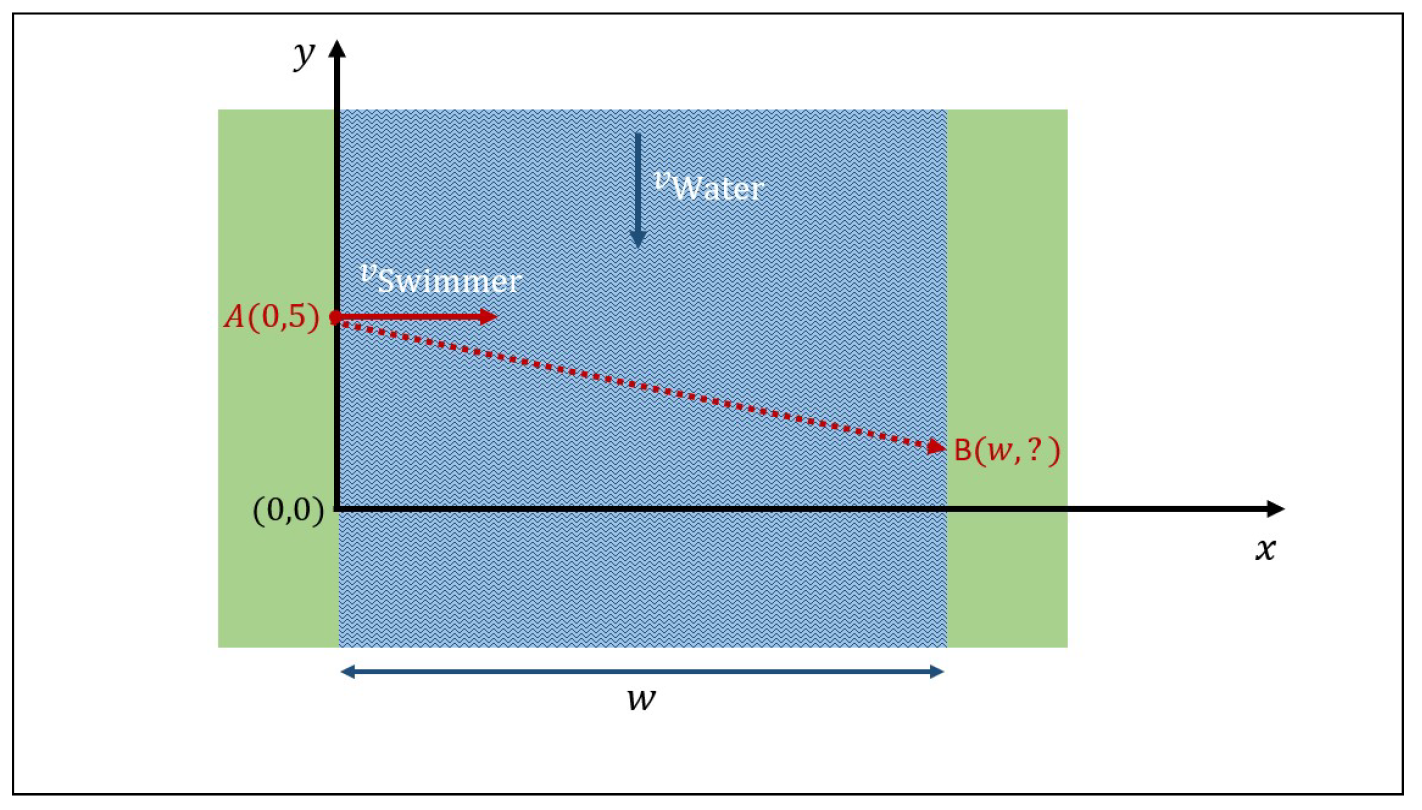
\includegraphics[width=0.9\textwidth]{../IMG/4H03.png} 
\end{figure}

\textit{Hints:
In this exercise you will need the multiplication * and division / operators.
The velocity $v$ is connected to the distance $d$ and the time $t$ via the following equation: $v = d/t$. Try solving for $d$ or $t$ to obtain equations to calculate time and distance given a specific velocity $v$.}\\[1cm]

